\section{Release Interfaces and Public Readouts}
\label{sec:method}

A public partition defines a compact naming task. We compare protected
regional votes, point votes and clipped heads, then hold their public readout
and annotation resources explicit. The regional mechanism is called SDD in
the reproducibility scripts; its direct NN readout is a naming classifier.
Figure~\ref{fig:pipeline} shows one deployment: the platform fits the
public partition, releases one protected regional matrix, decodes it jointly
with the counted labels, and, when verification is required, releases a
protected paired gain and a class histogram computed on client holdouts
before publishing the candidate or the public comparator; all releases share
one total budget.

% Schematic (no data): one deployment and its composed budget (vector figure, experiments/release-eab9-20261021/figure-source).
\begin{figure*}[t]
\centering
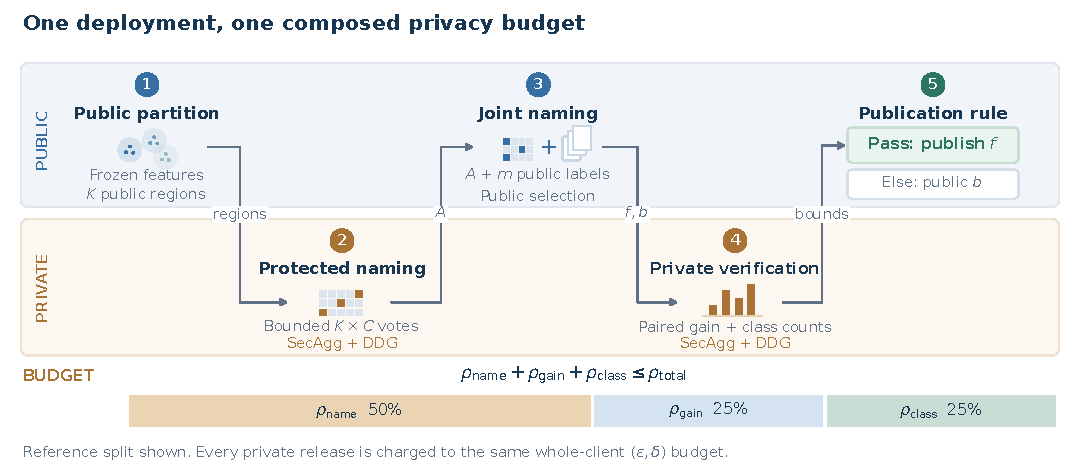
\includegraphics[width=.9\textwidth,trim=0 .19in 0 .40in,clip]{figures/fig-privacy-pipeline.pdf}
\Description{Public and private lanes of one deployment: public partition,
protected naming, joint naming, private verification and the publication
rule, with all private releases charged to one composed budget.}
\caption{One deployment across public and private operations. Protected
naming (2) and verification (4) consume the same whole-client privacy budget;
all operations on released statistics are public post-processing. Release
objects (regional votes, clipped head, pooled per-example votes) differ only
in step 2. The reference $50/25/25$ split is shown; other allocations change
the shares, not the composition rule.}
\label{fig:pipeline}
\end{figure*}



\subsection{A public partition for knowledge reuse}
\label{sec:method:cluster}

A fixed public extractor $g$ and public $K$-means form nonempty regions
$P_1,\ldots,P_K$, shared across rounds independently of private data.
Singleton regions recover per-example transfer; random partitions share the
sensitivity, so matched controls test geometry.

\subsection{One bounded opinion per region}
\label{sec:method:report}

For client model $f_i$, the regional posterior is
\begin{equation}
\bar R_i[k,\cdot]=\frac1{|P_k|}\sum_{x\in P_k}f_i(x)
\in\Delta^{C-1}.\label{eq:report}
\end{equation}
M votes for the largest component of $\bar R_i[k,\cdot]$.
R votes on $f_i(x_k^*)$, where $x_k^*$ is the public point nearest the
centroid: public representative queries followed by regional label propagation.
Both emit K one-hot rows over identical regions, matching sensitivity,
payload and partition quality.

\subsection{Noisy consensus and local learning}
\label{sec:method:agg}

Each client adds independent integer discrete-Gaussian shares to its quantised
report. The aggregate-only layer exposes $S=\sum_i(sR_i+G_i)$, and the server
projects $S/(sn)$ row-wise onto the simplex to obtain $A$.
For ordinary consensus, the target is
\begin{equation}
\hat y(x)=\arg\max_c A[k(x),c].\label{eq:targets}
\end{equation}
Centered decoding uses a fixed class-prior correction: with public region weights
$w_k=|P_k|$, subtract
$\pi_c=\sum_k w_k A[k,c]/\sum_k w_k$ before taking the arg-max.
It counters a common class preference under narrow local label coverage and
is the fixed zero-label decoder. Raw and coverage decoding are separate post-processing rules of the
same matrix; counted public labels can choose their use in joint naming.

\paragraph{Coverage-constrained decoding}
At taxonomy resolution $K=C$, a prespecified alternative is a one-to-one
assignment using the released matrix:
\begin{equation}
\hat\pi=\arg\max_{\pi\in\mathfrak S_C}\sum_k |P_k|A[k,\pi(k)],
\qquad \hat y(x)=\hat\pi(k(x)).
\label{eq:matching}
\end{equation}
Hungarian assignment solves it; it guarantees class coverage, while
correctness depends on whether the public regions support a one-to-one class
allocation. It needs no further private query or budget.
Soft-target controls reuse this protected matrix and are separately indexed.

The primary $T=1$ protocol trains each client privately before a single
release. We compare 60 and 180 pre-release SGD steps without proxy targets.
The naming-only contrasts allocate the full budget to this release;
Section~\ref{sec:private-verification} allocates part to private verification.
The $T=3$ extension trains for 60 steps before each release, mixing equal
private/proxy halves after the first. Releases 1/2 supervise later rounds;
release 3 follows the final local fit. All three consume budget. The extension couples later teachers to earlier names. A private-only
three-release control separates that feedback path from post-release averaging.

\paragraph{Two readouts from the same release}
The public classifier predicts
$\hat y(x)=\hat y_{\arg\min_k\|g(x)-\mu_k\|_2}$ using released regional
labels and fixed public centroids, post-processing publishable under the
transcript's whole-client DP; client models are not published. An optional
public softmax student trains for 180 server steps on the protected labels
only, with its public compute reported separately.

\paragraph{Payload and computation}
At $|P|=2000$, $C=10$, a $K=10/20$ release uses $100/200$ integer
coordinates, versus $20000$ per-example and $1280$ head coordinates, before
secret-sharing overhead. All server work after the release is public
post-processing. Row-wise
simplex projection of the $K\times C$ matrix costs $O(KC\log C)$ by
sorting; centered decoding costs $O(KC)$; the coverage-constrained and joint
decoders solve one $C\times C$ assignment in $O(C^3)$ time by the Hungarian
method. Exact LOO for joint assignment needs at most $C+1$ assignment solves
per weight (Proposition~\ref{prop:loo}), independent of $m$. Server cost thus
scales with $K$ and $C$, not with private data size.

Taxonomy resolution $K=C$, M and centered decoding specify the main
condition without public task labels; larger K and full-label configurations
are separate conditions.
